%%%%%%%%%%%%%%%%%%% EJERCICIO 13 %%%%%%

\textbf{Ejemplo 13}\\
Una persona debe pagar  10.000 COP con vencimiento en 3 meses, 15.000 COP a 10 meses y 20.000 COP con vencimiento en un año. Si hace un pago único de 45.000 COP, hallar la fecha en que debe hacerse, suponga una tasa del 18\% nominal anual mes vencido. Si consideramos la período focal en el período mes vencido 0:\\ \\
%\newpage %USAR SOLO SI EL SOLUCIÓN QUEDA SOLO Y ES NECESARIO BAJARLO A LA SIGUIENTE PAGINA
\textbf{Solución.}
%La tabla ira centrada
\begin{center}
  \renewcommand{\arraystretch}{1.5}% Margenes de las celdas
  %Creación de la cuadricula de 3 columnas
  \begin{longtable}[H]{|C{0.3\linewidth}|C{0.3\linewidth}|C{0.35\linewidth}|}
    %Creamos una linea horizontal
    \hline
    %Definimos el color de la primera fila
    \rowcolor[HTML]{FFB183}
    %%%%% INICIO ASIGNACIÓN PERíODO FOCAL %%%%%%%
    %%%%%%%%%% INICIO TITULO
    %Lo que se hace aquí es mezclar las 3 columnas en una sola
    \multicolumn{3}{|c|}{\cellcolor[HTML]{FFB183}\textbf{1. Asignación período focal}}                                                                                          \\ \hline
    \multicolumn{3}{|c|}{\textbf{ $pf : \textit{ 0 pmv} $}}                                                                                                      \\ \hline
    %%%%%%%%%% FIN TITULO
    %%%%% INICIO DECLARACIÓN DE VARIABLES %%%%%%%
    %%%%%%%%%% INICIO TITULO
    %Lo que se hace aquí es mezclar las 3 columnas en una sola
    \multicolumn{3}{|c|}{\cellcolor[HTML]{FFB183}\textbf{2. Declaración de variables}} \\ \hline
    \multicolumn{3}{|c|}{\cellcolor[HTML]{FFB183}\textbf{Deuda Inicial}} \\ \hline
    %%%%%%%%%% FIN TITULO
    %%%%%%%%%% INICIO SUBTITULO
    \cellcolor[HTML]{FFB183}\textbf{Valores monetarios}    & 
    \cellcolor[HTML]{FFB183}\textbf{Valores no monetarios} &
    \cellcolor[HTML]{FFB183}\textbf{Incógnitas}  \\ \hline
    %%%%%%%%%% FIN SUBTITULO
    %%%%%%%%%% INICIO DE MATEMÁTICAS
    %Cada & hace referencia al paso de la siguiente columna

    $F_{1} =10.000$ COP & $n_{1} = 3 \textit{ pmv} $ & \\
    $F_{2} = 15.000$ COP & $n_{2} = 10 \textit{ pmv} $ & \\
    $F_{3} =20.000$ COP & $n_{3}= 12 \textit{ pmv}  $ & \\ \hline
    
    %%%%%%%%%% INICIO TITULO
    \multicolumn{3}{|c|}{\cellcolor[HTML]{FFB183}\textbf{Deuda Inicial}} \\ \hline
    %%%%%%%%%% FIN TITULO
    %%%%%%%%%% INICIO SUBTITULO
    \cellcolor[HTML]{FFB183}\textbf{Valores monetarios}    & 
    \cellcolor[HTML]{FFB183}\textbf{Valores no monetarios} &
    \cellcolor[HTML]{FFB183}\textbf{Incógnitas}  \\ \hline
    %%%%%%%%%% FIN SUBTITULO
    %Cada & hace referencia al paso de la siguiente columna
    $F_{4} =45.000$ COP & $j= 18\% \textit{ namv} $ & $n_{4} = ¿? \textit{ pmv} $ \\
    & $m = 12 \textit{ pmv} $ & \\
    & $i = \frac{18\% \textit{ namv}}{12 \textit{ pmv}} = 1,5\% \textit{ pmv} $ & \\ \hline
    %%%%%%%%%% FIN DE MATEMÁTICAS
    %%%%% FIN DECLARACIÓN DE VARIABLES
    %%%%% INICIO FLUJO DE CAJA
    \rowcolor[HTML]{FFB183}
    \multicolumn{3}{|c|}{\cellcolor[HTML]{FFB183}\textbf{3. Diagrama de flujo de caja}}                                                                                         \\ \hline
    %Mezclamos 3 columnas y pondremos el dibujo
    %%%%%%%%%%%%% INSERCIÓN DE LA IMAGEN
    %Deberán descargar las imágenes respectivas del drive y pegarlas en la carpeta
    %n_capitulo/img/ejemplos/1/capitulo1ejemplo1.pdf  (el /1/ es el numero del ejemplo)
    \multicolumn{3}{|c|}{ 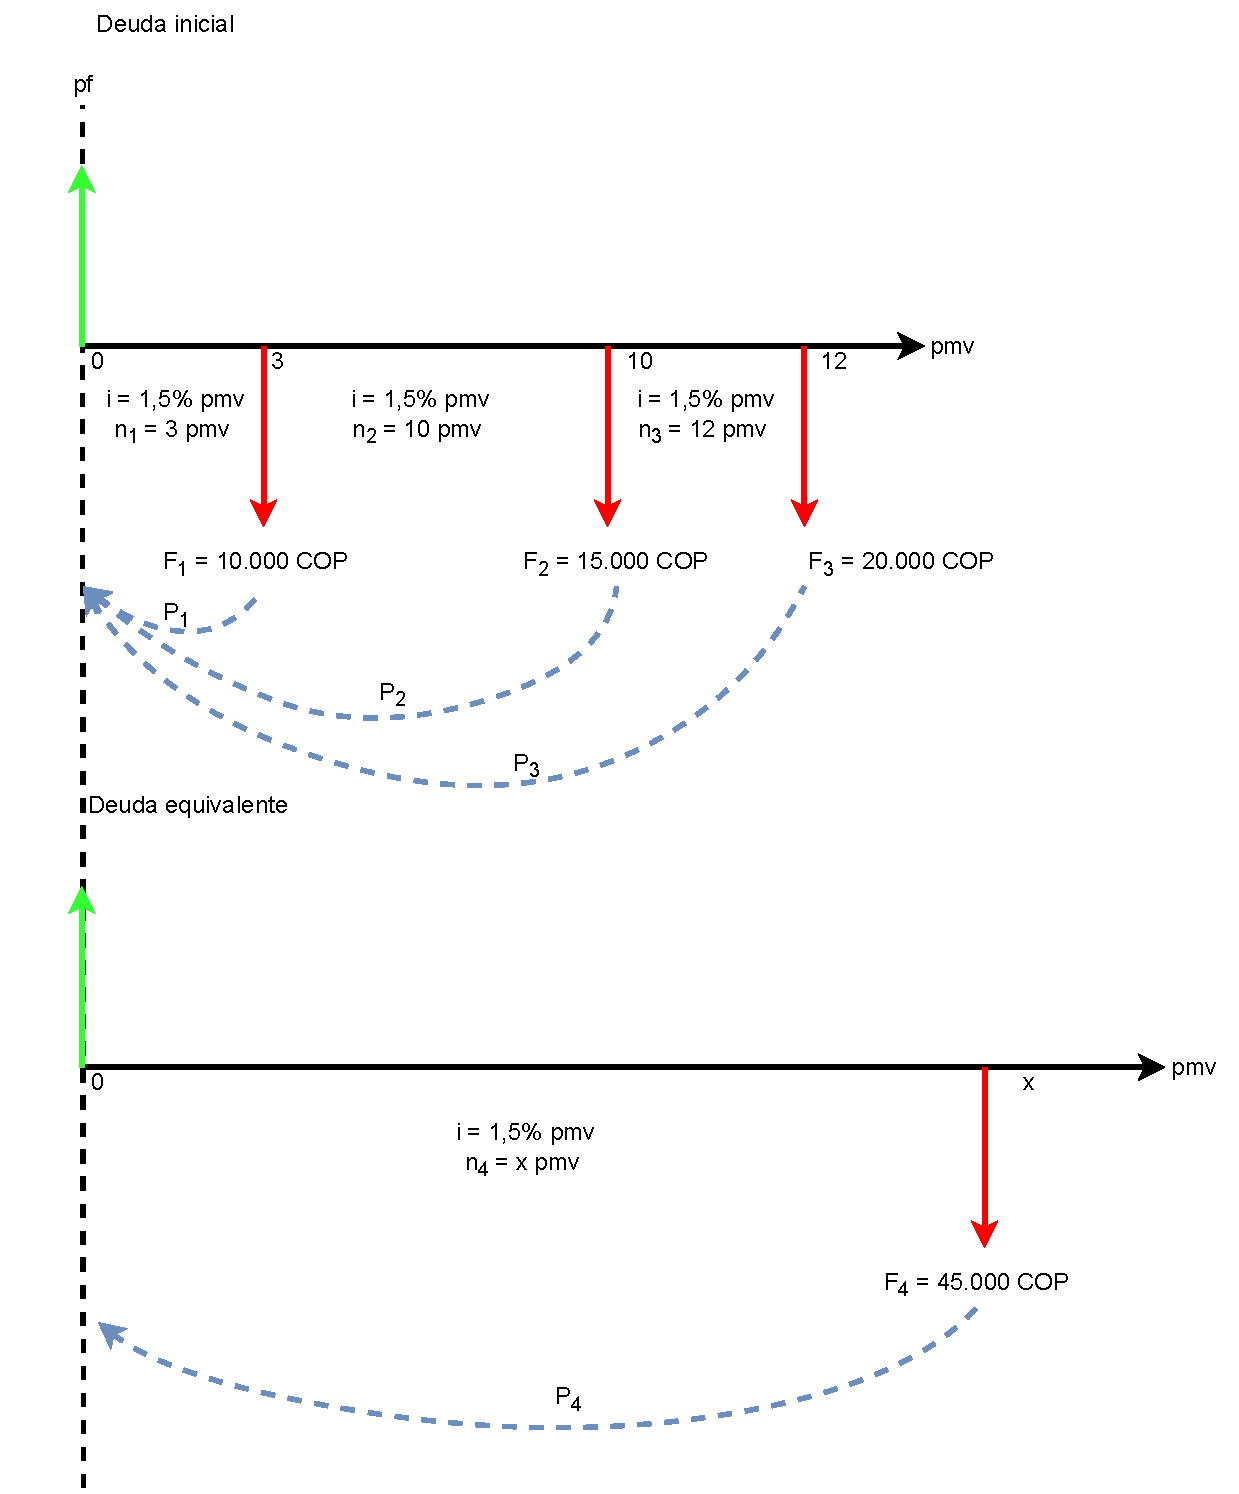
\includegraphics[trim=-5 -5 -5 -5 , scale=0.5]{2_Capitulo/img/ejemplos/14/Ejemplo 13Ver.pdf} }
    \\ \hline
    %%%%%%%%%%%%% FIN INSERCIÓN DE IMAGEN
    %%%%%FIN FLUJO DE CAJA



    %%%%% INICIO DECLARACIÓN FORMULAS
    %%%%%%%%%%% INICIO TITULO
    \rowcolor[HTML]{FFB183}
    \multicolumn{3}{|c|}{\cellcolor[HTML]{FFB183}\textbf{4. Declaración de fórmulas}}                                                                                           \\ \hline
    %%%%%%%%%%% FIN TITULO
    %%%%%%%%%%% INICIO MATEMÁTICAS

    \multicolumn{3}{c|}{$P_{1} + P_{2} + P_{3} = P_{4} \hspace{0.3cm} \textit{ Ecuación de equivalencia}$} \\
    \multicolumn{3}{c|}{$P = F(1+i)^{-n} \hspace{0.3cm} \hspace{0.3cm} \textit{Valor presente}$ } \\ \hline
    %%%%%%%%%% FIN MATEMÁTICAS
    %%%%%% INICIO DESARROLLO MATEMÁTICO
    %%%%%%%%%%INICIO TITULO
    \rowcolor[HTML]{FFB183}
    \multicolumn{3}{|c|}{\cellcolor[HTML]{FFB183}\textbf{5. Desarrollo matemático}} \\ \hline
    %%%%%%%%%% FIN TITULO
    %%%%%%%%%% INICIO MATEMÁTICAS

    \multicolumn{3}{|c|}{$10{.}000 \textit{ COP} (1 + 0,015)^{-3}$ + $15{.}000 \textit{ COP} (1 + 0,015)^{-10}$} \\
    \multicolumn{3}{|c|}{+ $20{.}000 \textit{ COP} ( 1 + 0,015)^{-12} = 45{.}000 \textit{ COP} ( 1 + 0,015)^{-n_{4}} $} \\
    \multicolumn{3}{|c|}{$39{.}215.92 = 45{.}000 \textit{ COP} ( 1.015)^{-n_{4}} $} \\
    \multicolumn{3}{|c|}{$\frac{39{.}215.92}{45{.}000 \textit{ COP}} = 1.015^{-n_{4}} $} \\
    \multicolumn{3}{|c|}{$0.87146 = 1.015^{-n_{4}} $} \\
    \multicolumn{3}{|c|}{$\log(0.87146) = \log(1.015^{-n_{4}}) $} \\
    \multicolumn{3}{|c|}{$\log(0.87146) = -n_{4} \log(1.015) $} \\
    \multicolumn{3}{|c|}{$\frac{\log(0.87146)}{-\log(1.015)} = n_{4} $} \\
    \multicolumn{3}{|c|}{$n_{4} = 9.24059 \textit{ pmv} \approx  9 \textit{ meses y } 7 \textit{ días}$} \\ \hline
    %%%%%%%%%% FIN MATEMÁTICAS
    %%%%%% FIN DESARROLLO MATEMÁTICO
    %%%%%% INICIO RESPUESTA
    
    %%%%%%%%%%INICIO TITULO
    \multicolumn{3}{|c|}{\cellcolor[HTML]{FFB183}\textbf{6. Respuesta}} \\ \hline
    \multicolumn{3}{|c|}{$n_{4} \approx 9 \textit{ meses y } 7 \textit{ días } $}                                                                                                       \\ \hline
    %%%%%%%%%% FIN TITULO
    %%%%%%%%%% INICIO RESPUESTA MATEMÁTICA
    \multicolumn{3}{|c|}{

      \begin{minipage}[t][0.07\textheight][c]{0.8\columnwidth}
       \centering
        $n_{4} = 9,24059 \textit{ pmv} \approx t = 9 \textit{ meses y }  7 \textit{ días.} $
      \end{minipage}
    }                                                                                                                                                                           \\ \hline


    %%%%%%%%%% FIN MATEMÁTICAS
    %%%%%% FIN RESPUESTA
  \end{longtable}
  %Se crean dos lineas en blanco para que no quede el siguiente texto tan pegado
  %\newline \newline %USARLO SI CREES QUE ES NECESARIO
\end{center}
%%%%%%%%%%%%%%%%%%%%%%%%%%FIN EJERCICIO 13 %%%%%%%%%%%%%%%%%%%%%%%%%%%